\documentclass[]{standalone}

% More defined colors
\usepackage[dvipsnames]{xcolor}
\definecolor{royal_blue}{RGB}{0,83,214}
\definecolor{gray_black}{RGB}{18,54,147}

\usepackage{tikz}
\usetikzlibrary{positioning, shapes.geometric, calc, arrows.meta}

\tikzstyle{block} = [
    rectangle, rounded corners, text centered, 
    minimum width=0.5cm, minimum height=0.5cm,
    text width=4cm, line width=0.1mm, inner sep=2mm,
    draw=gray_black, fill=white, text=royal_blue,
]

\tikzstyle{tablecell} = [
    rectangle, line width=0.5mm, 
    minimum width=0.85cm, minimum height=0.85cm,
    inner sep=0mm,
]

\tikzstyle{sum} = [
    circle, minimum width = 4mm, minimum height = 4mm, draw=gray_black, fill = white, inner sep = 0cm, text = royal_blue
]

% \tikzstyle{heavyarrow} = [very thick,->,>=stealth]
\tikzstyle{arrow} = [thick, -latex, gray_black]


\begin{document}
 
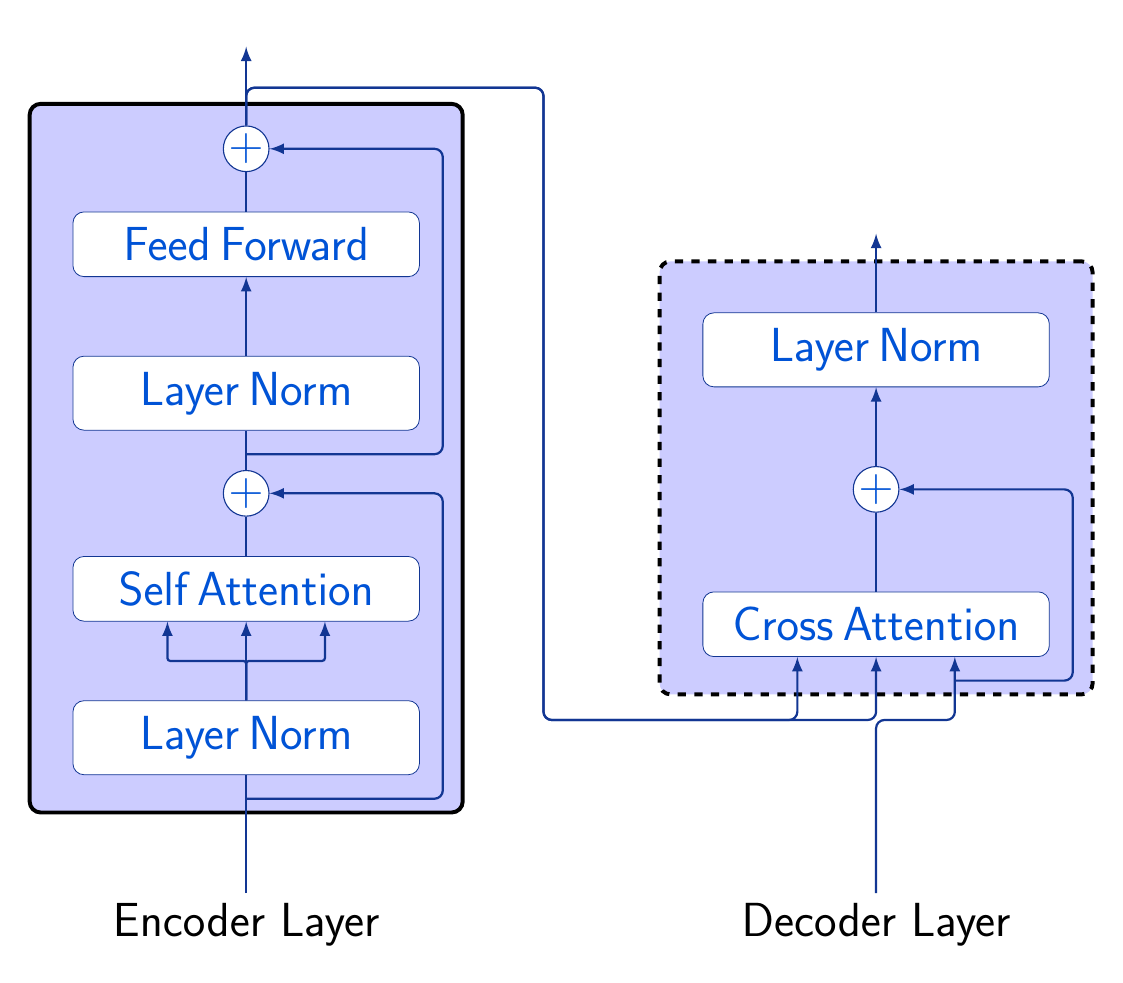
\begin{tikzpicture}

    % encoder layer nodes
    \node[] (encoder_layer_text) at (0,0) {\sffamily \LARGE Encoder Layer};
    \node[block, minimum width=5.5cm, minimum height=9cm, line width=0.5mm, draw=black, fill=blue!20] (encoder_layer_outline) [above=of encoder_layer_text] {};
    \node[block] (layer_norm1) [above= 1.5cm of encoder_layer_text] {\sffamily \LARGE Layer Norm};
    \node[block] (self_attn) [above=of layer_norm1] {\sffamily \LARGE Self Attention};
    \node[sum] (residual1) [above=0.5cm of self_attn] {\LARGE +};
    \node[block] (layer_norm2) [above=0.5cm of residual1] {\sffamily \LARGE Layer Norm};
    \node[block] (mlp) [above=of layer_norm2] {\sffamily \LARGE Feed Forward};
    \node[sum] (residual2) [above=0.5cm of mlp] {\LARGE +};
    \node[] (encoder_output) [above= 1.cm of residual2] {};
    
    % decoder layer nodes
    \node[] (decoder_layer_text) at (8,0) {\sffamily \LARGE Decoder Layer};
    \node[block, minimum width=5.5cm, minimum height=5.5cm, line width=0.5mm, draw=black, dashed, fill=blue!20] (decoder_layer_outline) [above=2.5cm of decoder_layer_text] {};
    \node[block] (cross_attn) [above= 3cm of decoder_layer_text] {\sffamily \LARGE Cross Attention};
    \node[sum] (decoder_residual) [above=of cross_attn] {\LARGE +};
    \node[block] (decoder_layer_norm) [above=of decoder_residual] {\sffamily \LARGE Layer Norm};
    \node[] (decoder_output) [above= 1.cm of decoder_layer_norm] {};
    
    % arrows in encoder layer
    \draw[arrow, -] (encoder_layer_text) to (layer_norm1);
    \draw[arrow] (layer_norm1) to (self_attn);

    \coordinate[below=0.5cm of self_attn.south, xshift=-1cm] (anchor8);
    \coordinate[below=0cm of self_attn.south, xshift=-1cm] (anchor9);
    \draw[arrow, rounded corners=1pt] (layer_norm1.north) |- (anchor8) to (anchor9);
    \coordinate[below=0.5cm of self_attn.south, xshift=1cm] (anchor10);
    \coordinate[below=0cm of self_attn.south, xshift=1cm] (anchor11);
    \draw[arrow, rounded corners=1pt] (layer_norm1.north) |- (anchor10) to (anchor11);

    \coordinate[below=0.3cm of layer_norm1.south] (anchor12);
    \coordinate[right=2cm of residual1.east, xshift=0.2cm] (anchor13);
    \draw[arrow, rounded corners=3pt] (anchor12) -| (anchor13) to (residual1.east);

    \coordinate[below=0.3cm of layer_norm2.south] (anchor14);
    \coordinate[right=2cm of residual2.east, xshift=0.2cm] (anchor15);
    \draw[arrow, rounded corners=3pt] (anchor14) -| (anchor15) to (residual2.east);

    \draw[arrow, -] (self_attn) to (residual1);
    \draw[arrow, -] (residual1) to (layer_norm2);
    \draw[arrow] (layer_norm2) to (mlp);
    \draw[arrow, -] (mlp) to (residual2);
    \draw[arrow] (residual2) to (encoder_output);

    % arrows from encoder layer to decoder layer
    \coordinate[above right= 0.8cm of residual2, xshift=3cm] (anchor1);
    \coordinate[below=0.8cm of cross_attn.south, xshift=-1cm] (anchor2);
    \coordinate[below=0cm of cross_attn.south, xshift=-1cm] (anchor3);
    \draw[arrow, rounded corners=3pt] (residual2.north) |- (anchor1) |- (anchor2) to (anchor3);
    \coordinate[below=0.8cm of cross_attn.south] (anchor4);
    \coordinate[below=0cm of cross_attn.south] (anchor5);
    \draw[arrow, rounded corners=3pt] (residual2.north) |- (anchor1) |- (anchor4) to (anchor5);

    % arrows in decoder layer
    \coordinate[below=0.8cm of cross_attn.south, xshift=1cm] (anchor6);
    \coordinate[below=0cm of cross_attn.south, xshift=1cm] (anchor7);
    \draw[arrow, rounded corners=3pt] (decoder_layer_text.north) |- (anchor6) to (anchor7);

    \coordinate[below=0.3cm of cross_attn.south, xshift=1cm] (anchor16);
    \coordinate[right=2cm of decoder_residual.east, xshift=0.2cm] (anchor17);
    \draw[arrow, rounded corners=3pt] (anchor16) -| (anchor17) to (decoder_residual.east);

    \draw[arrow, -] (cross_attn) to (decoder_residual);
    \draw[arrow] (decoder_residual) to (decoder_layer_norm);
    \draw[arrow] (decoder_layer_norm) to (decoder_output);
\end{tikzpicture}

\end{document}